\chapter{Stand der Technik}
Die Entwicklung einer neuen Messtechnik für das Fahrrad und den Flying Suit stellt eine komplexe Aufgabe da.
Dies beinhaltet die Planung und Bestellung nötiger Materialien und die Anbringung dieser am jeweiligen Aufbau.
Um sicherzustellen, dass die zu entwickelnde technische Umsetzung möglich ist, wurde das Zusammenspiel von Node und Dehnungsmessstreifen zunächst am einfacheren Aufbau eines Biegebalkens getestet.


\section{Biegebalken (Menzel)}
\subsection{Aufbau des Biegebalkens}
Auf der Ober- und Unterseite des Biegebalkens sind Dehnungsmessstreifen angebracht um die beim aufbringen eines Gewichts entstehende Dehnung messen zu können.
Dies wurde mit verschiedenen Gewichten und in verschiedenen Einheiten durchgeführt.
\begin{figure}[h]
    \begin{center}
        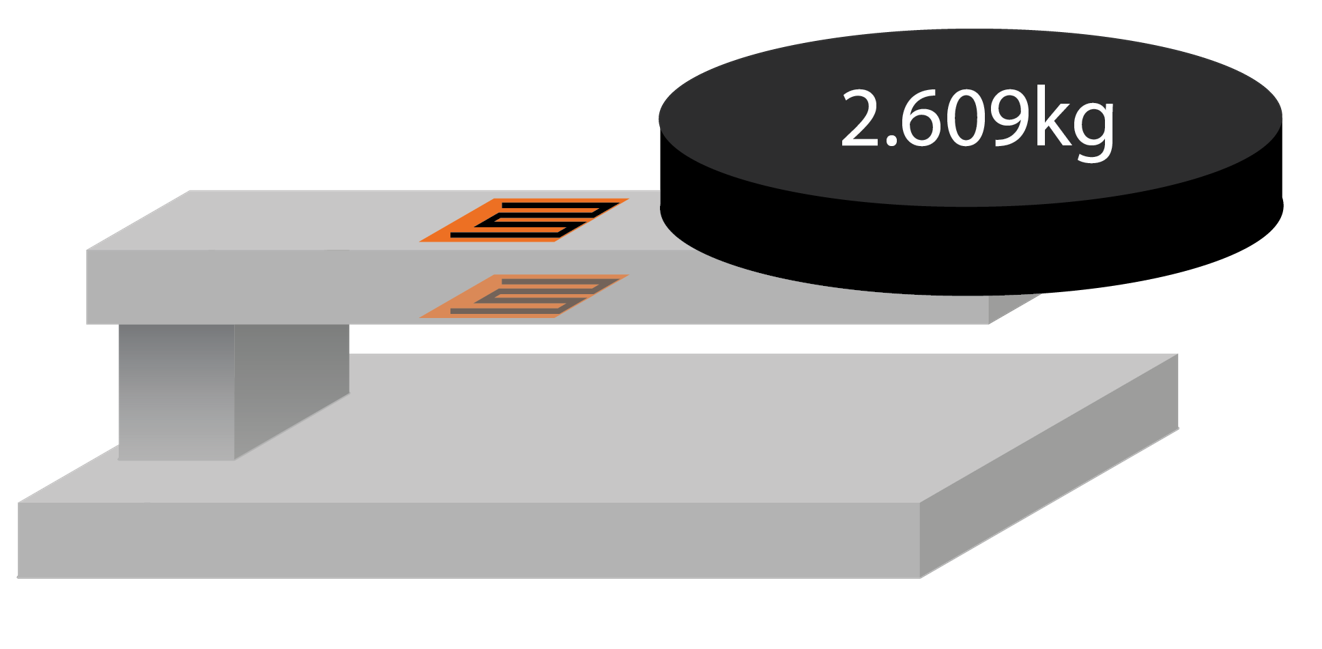
\includegraphics[width=0.5\textwidth, keepaspectratio]{biegebalken_grafik.png}
        \caption[Biegebalken Schema (Abbildungsverzeichnis)]{Biegebalken Schema
        %\cite{VLInkManual}
        }
        \label{fig:biegebalkenschema}
    \end{center}
\end{figure}
\subsection{Berechnung der Sensitivity}
Um eine Messung am Biegebalken durchführen zu können wurde zunächst die Sensitivity mathematisch berechnet.
Sie basierst auf der Geometrie des Biegebalkens, sowie des zu erwartendem maximalen Gewicht und wird als Parameter in SensorConnect eingegeben.
Sie stellt den gemessenen Wert in mV/V bei Maximalbelastung dar.
Aufgrund der einfachen Geometrie des Biegebalkens ist dies ein wichtiger Schritt, bevor diese für die komplexere Geometrie des Fahrradlenkers oder des Gestells des Flying Suits berechnet wird.

In der folgenden Berechnung wird für den Parameter n der Wert 2 verwendet, da es sich um die Anzahl der angebrachten DMS und die daraus resultierende Brückenkonfiguration handelt.
Der Parameter k ist durch die verwendeten DMS gegeben. Als maximale Last dient eine Hantelscheibe mit einem Gewicht von 2.609kg.



Maße des Biegebalkens:
\[
l = 117 \text{ mm}, \quad b = 19.8 \text{ mm}, \quad h = 2.94 \text{ mm}
\]
Maximale Last:
\[
M = 2.609 \text{ kg}
\]

\subsection*{Berechnung des Widerstandsmoments}
\[
W_x = \frac{b h^2}{6}
\]
Einsetzen der Werte:
\[
W_x = \frac{19.8 \times 2.94^2}{6} = 28.52 \text{ mm}^3
\]

\subsection*{Berechnung des Biegemoments}
\[
M_b = F \times l
\]
\[
M_b = 2.609 \times 9.81 \times 117mm = 2994.53 \text{ Nmm}
\]

\subsection*{Berechnung der Spannung}
\[
\sigma = \frac{M_b}{W_x}
\]
\[
\sigma = \frac{2994.53}{28.52} = 104.99 \text{ N/mm}^2
\]

\subsection*{Berechnung der Dehnung}
\[
\varepsilon = \frac{\sigma}{E}
\]
Mit \(E = 210000 \text{ N/mm}^2\):
\[
\varepsilon = \frac{104.99}{210000} = 0.499\times 10^{-3}
\]

\subsection*{Berechnung der Brückenausgabe}
\[
\frac{U_M}{U_B} = \frac{n}{4} \times k \times \varepsilon
\]
Mit \( n = 2 \), \( k = 2.01 \):
\[
\frac{U_M}{U_B} = \frac{2}{4} \times 2.01 \times 0.499 \times 10^{-3}
\]
\[
\frac{U_M}{U_B} = 0.000502 \text{ V/V} = 0.5 \text{ mV/V}
\]

Mit der berechneten Sensitivity wurden mehrere Messungen durchgeführt.